\chapter{Low Level Vision}
La low level vision si basa su algoritmi che ricalcano proprietà matematiche per estrarre informazioni utili dalle immagini. Questa branca della computer vision raramente fa uso di intelligenza artificiale e si adatta bene a contesti semplici e controllati come la visione industriale.

La low level vision ha come obbiettivo quello di estrarre delle regioni di interessa dalle immagini, evidenziare bordi e punti di interesse di un'immagine.

\section{Segmentation}
Vogliamo suddividere l'immagine in aree di interesse, cioè creare una maschera che ritagli delle aree dell'immagine semanticamente differenti. La maschera più semplice a cui possiamo pensare ha solo 2 livelli e permette di ottenere un'immagine binarizzata in cui distinguiamo la ragione di interesse dallo sfondo.

\subsection{Thresholding}
È uno dei metodi più intuitivi per fare segmentazione di un'immagine, è molto utilizzato date le se buone proprietà e la pochissima complessità computazionale. Il thresholding permette di dividere i pixel in regioni basandosi sulle proprietà dei pixel stessi.

La forma più semplice di thresholding consiste nel decidere una soglia $T$ e dividere i pixel con intensità minore di $T$ da quelli con intensità maggiore; questo approccio è detto \textbf{thresholding globale}. Se la soglia cambia parliamo invece di thresholding variabile, questo si divide in \textbf{thresholding locale} se $T$ dipende dalle caratteristicche del vicinato del pixel in esame, oppure \textbf{thresholding adattativo} se $T$ dipende dalla posizione nell'immagine.

Lo scopo del thresholding è quello di risolvere un problema decisionale statistico. Vogliamo minimizzare il numero di pixel etichettati nel modo sbagliato.  

Questo significa conoscere la distribuzione dei pixel che rappresentano lo sfondo e la distribuzione dei pixel che rappresentano il soggetto. Stimare le PDF è un problema tutt'altro che semplice, e anche se assumiamo siano distribuzioni normali trovare la soglia ccorretta non è semplice.

\subsubsection{Thresholding globale semplice}
Questo metodo è adatto quando le distribuzioni di pixel sono chiaramente bimodali e la separazione è relativamente facile. La soglia $T$ viene trovata iterativamente raffinando delle stime. L'algoritmo seguito per trovare $T$ è il seguente:
\vspace{.5cm}

\begin{algorithmic}
	\Function{BasicThresholding}{ }
		\State $\Delta T \gets \infty$
		\State $T \gets T_{init}$
		\While{$\Delta T < \Delta T_{min}$}
			\State $G_1 \gets$ \Call{PixelLess}{$T$}
			\State $G_2 \gets$ \Call{PixelGreather}{$T$}
			\State $m_1 \gets$ \Call{IntensityMean}{$G_1$}
			\State $m_2 \gets$ \Call{IntensityMean}{$G_1$}
			\State $T_{new} \gets \frac{m_1 + m_2}{2}$
			\State $\Delta T \gets |T - T_{new}|$
			\State $T \gets T_{new}$
		\EndWhile
	\EndFunction    
\end{algorithmic}

\subsubsection{Thresholding di Otsu}
Al posto di minimizzare i pixel etichettati in modo sbagliato ci concentriamo sul massimizzare la differenza tra le due classi di pixel che separiamo. Questo consiste nel massimizzare la varianza inter-classe (tra le classi).

Il metodo di Otsu è vantaggioso anche perché permette di lavorare unicamente con l'istogramma, che è facile da ottenere e permette di costruire un algoritmo molto efficiente dal punto di vista computazionale.

Avendo $L$ livelli di intensità, un immagine di dimensione $N\times M$ e chiamando $n_i$ il numero di pixel aventi intensità $i$ possiamo la probabilità che un pixel dell'immagine abbia intensità $i$ cioè $p_i = n_i/MN$.

Se scegliamo una soglia $k$ possiamo ora derivare la probabilità che un certo pixel appartenga alla prima ($c_1$) o alla seconda ($c_2$) classe:
\begin{align}
	P_1(k) & = \sum_{i = 0}^{k} p_i\\
	P_2(k) & = \sum_{i = k+1}^{L-1} p_i = 1-P_1
\end{align}
Possiamo calcolare l'intensità media dei pixel in $c_1$, in $c_2$ e la media cumulativa fino al livello $k$ come:
\begin{align}
	m_1(k) & = \sum_{i = 0}^{k} iP(i/c_1) = \frac{1}{P_1} \sum_{i = 0}^{k}ip_i\\
	m_2(k) & = \sum_{i = k+1}^{L-1} iP(i/c_2) = \frac{1}{P_2} \sum_{i = k+1}^{L-1}ip_i\\
	m(k) & = \sum_{i = 0}^{k} ip_i
\end{align}
Definiamo ora la varianza inter-classe come  :
\begin{align}
	\sigma^2_G & = P_1(m_1 - m_G)^2 + P_2(m_2 - m_G)^2= \notag \\
	& = P_1 P_2(m_1-m_2)= \notag \\
	& = \frac{(m_gP_1 - m)^2}{P_1 P_2}
\end{align}
Possiamo ricavare il valore ottimo per la soglia $k^*$ che permette di massimizzare la varianza
\begin{equation}
	\sigma^2_B(k^*) = \underset{0\leq k \leq L-1}{\max} \sigma^2_B(k) = \underset{0\leq k \leq L-1}{\max} \left( \frac{\left[m_gP_1(k) - m(k)\right]^2}{P_1(k)P_2(k)}\right)
\end{equation}

\subsubsection{Migliorare il thresholding globale}
Per migliorare il thresholding globale possiamo usare diverse tecniche:
\begin{enumerate}
	\item moothing dell'immagine;
	\item usare i bordi per individuare la soglia corretta.
\end{enumerate}
\newpage
La prima tecnica consiste nell'applicare un filtro passa basso, facendo \textbf{blurring dell'immagine} possiamo:
\begin{itemize}
	\item ridurre il rumore;
	\item scegliere la dimensione dei dettagli da evidenziare;
	\item passare da un istogramma confuso a uno bimodale.
\end{itemize}

La seconda tecnica si basa sul fatto che tipicamente siamo interessati a separare il soggetto dallo sfondo, se il soggetto ha dei bordi sufficientemente marcati possiamo evidenziarli (ad esempio con il laplaciano) e trovare la soglia di threshold ottima solo sui pixel di bordo. Per fare questo costruiamo una maschera a partire dal laplaciano e la usiamo per selezionare i bordi dell'immagine di partenza. Uno volta trovata la soglia ottima possiamo applicarla a tutta l'immagine.

\subsubsection{Threshold variabile}
\begin{wrapfigure}[20]{r}{.35\linewidth}
	\vspace{-.8cm}
	\centering
	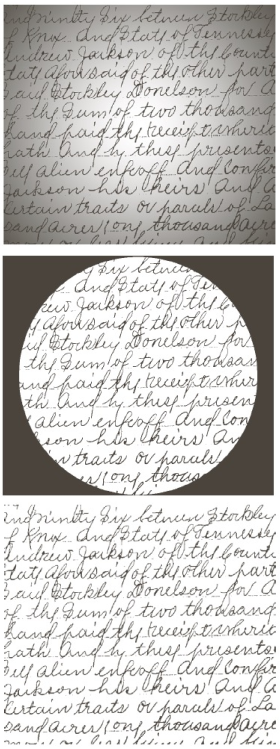
\includegraphics[width=.95\linewidth]{Picture/Moving_Average_Threshold}
\end{wrapfigure}
Compensa un'illuminazione non uniforme definendo per ogni pixel una soglia attraverso strumenti statistici.

Esempi di definizione di soglia sono:
\begin{align*}
	T_{xy} &= a\sigma{xy} +bm_{xy}\\
	T_{xy} &= a\sigma{xy}+bm
\end{align*}

Un esempio più complicato di statistica per scegliere la soglia è quello della \textbf{media mobile}; questa consiste nello scandire l'immagine per riga e risulta particolarmente utile per il riconoscimento del testo. Definiamo la media al passo $k+1$ come
\begin{align}
	m(k+1) &= \frac{1}{n}\sum_{i=k+2-n}^{k+1} z_i =\\ \notag
	               &=m(k)\frac{z_{k+i} - z_{k-n}}{n}
\end{align}
Dove $z_i$ è l'intensità del pixel $i$ e $m(1) = z_1 / n$
Nella figura vediamo l'immagine originale, quella binarizzata col metodo di Otsu e infine qella con la media mobile.

\subsection{Region growing}
Costruiamo le regioni di interesse a partire da un punto che sicuramente vi appartiene (\textbf{seed}) e facciamo crescere la regione aggiungendo pixel che soddisfano una determinata proprietà $Q$.

La parte più complessa di questa procedure è quella di individuare i seed, per fare questo può essere necessario esaminare tutti i pixel dell'immagine per cercare candidati adatti.

Una volta individuati i seed l'algoritmo di region growing è relativamente semplice: per ogni seed individuato si invoca la seguente funzione ricorsiva:
\vspace{.2cm}
\begin{algorithmic}
	\Function{RegionGrowing}{$seed$}
		\State $neighbors \gets $ \Call{8-Connected}{$seed$}
		\ForAll{$pixel$ \textbf{in} $neighbors$}
			\If{\Call{Satisfy}{$Q$,$pixel$}}
				\State $pixel.valid \gets \text{true}$
				\State \Call{RegionGrowing}{$pixel$} 
			\EndIf
		\EndFor
	\EndFunction    
\end{algorithmic}
\vspace{.2cm}
Al termine di ogni chiamata si ottiene una nuova regione di pixel marcati come validi, a questa regione si può poi dare un'etichetta per costruire una maschera.

\subsection{Region splitting and merging}
Questa procedura permette di dividere l'immagine in regioni ricorsivamente più piccole e di raggruppare le regioni adiacenti che rispettano una data proprietà $Q$. La struttura che descrive l'immagine al termine della procedura è un \textbf{quad-tree}; il quad-tree è una struttura molto compatta di rappresentare l'informazione e consente di decidere a priori la grana con cui ricostruire le regini di interesse.

La procedure si divide un due parti, la prima si occupa di dividere le regioni $R$ in sotto-regioni, la seconda di unire le sotto-regioni se entrambe rispettano una proprietà.
\vspace{.1cm}
\begin{algorithmic}
	\Function{Split}{$R$}
		\If{(\textbf{not }\Call{Satisfy}{$Q$,$R$}) \textbf{and} ($R > R_{min}$)}
			\State $R_1$, $R_2$, $R_3$, $R_4$ $\gets \Call{Divide}{R}$
			\State \Call{Split}{$R_1$}, \Call{Split}{$R_2$}, \Call{Split}{$R_3$}, \Call{Split}{$R_4$}
		\EndIf
	\EndFunction    
\end{algorithmic}
\newpage

\begin{algorithmic}
	\Function{Merge}{$region\_set\ R$}
	\DoWhile
		\State $old\_R \gets R$
		\ForAll{$R_a \in R$}
			\ForAll{$R_b \in \Call{Adjacent}{R_a}$}
				\If{\Call{Satisfay}{$Q$,$R_a\cup R_b$}}
					\State$R_{ab} = R_a\cup R_b$
					\State $R  \gets R/\{R_a, R_b\} \cup R_{ab}$
				\EndIf
			\EndFor
		\EndFor
	\EndDoWhile{$R \neq old\_R$}
	\EndFunction    
\end{algorithmic}

\section{Feature Extraction}
Lo scopo della feature extraction è quello di estrarre caratteristiche utili da un'immagine. Non esiste una definizione precisa  e condivisa di cosa sia una feature; in generale le caratteristiche che cerchiamo dipendono dall'appliccazione e dall'elaborazione che seguirà l'estrazione.

A prescindere da cosa consideriamo feature il processo di estrazione si divide un due fasi principali:
\begin{enumerate}
	\item feature detection;
	\item feature description.
\end{enumerate}
Vogliamo cioè non solo individuare le caratteristiche utili, ma essere in grado di descriverle per trovare similitudini e differenze tra feature estratte da diversi punti dell'immagine o tra immagini diverse.

\subsection{Edge Detection}
Sviluppiamo dei metodi per identificare i bordi che siano più robusti e affidabili della semplice derivata (gradiente o laplaciano).

\subsubsection{Marr-Hildreth edge detector}
Questo metodo è molto semplice, non assicura risultati ottimi ma permette di migliorare le prestazioni del detector rispetto al semplice laplaciano. L'idea è che il rumore presente in un immagine può generare falsi positivi, possiamo rimuovere parte di questo disturbo con un filtro gaussiano passa basso. Il filtro ha anche lo scopo di selezionare la dimensione minima dei bordi che vogliamo tenere in considerazione. La procedura per estrarre i bordi è la seguente:
\begin{enumerate}
	\item filtrare l'immagine con un filtro gaussiano passa basso $n\times n$ ($G(x,y)$);
	\item applicare l'operatore laplaciano ($\nabla^2$) al risultato;
	\item trovare i punti di zero crossing.
\end{enumerate}
Possiamo scrivere l'immagine ottenuta al passo 2 come 
\begin{equation}
	g(x,y) = \nabla^2\left[G(x,y)*f(x,y)\right]
\end{equation}
Il punto chiave di questa procedura è quello considerare bordi solo i pixel che si trovano a metà tra due pixel con segno opposto (zero crossing), questo unito al fatto di poter scegliere una soglia minima per il modulo della differenza dei pixel di segno opposto permette di ottenere buoni risultati etichettando bordi fini e precisi.

\subsubsection{Canny edge detector}
È l'algoritmo per l'estrazione dei bordi più complesso, ma che da risultati migliori. Questo metodo ha 3 obbiettivi:
\begin{itemize}
	\item \textbf{basso tasso d'errore}: tutti i bordi devono essere identificati;
	\item \textbf{bordi ben localizzati}: la distanza tra il punto etichettato come bordo e il bordo reale deve essere la minima possibile
	\item \textbf{single point response}: per ogni punto del bordo deve essere etichettato un solo punto, cioè non si devono etichettare i massimi locali nelle prossimità di un  bordo.
\end{itemize}

L'algoritmo è diviso in 4 fasi principali:
\begin{enumerate}
	\item Smoothing dell'immagine con un filtro gaussiano;
	\item Calcolo del gradiente con angolo e modulo;
	\item applicazione della Non Maxima Suppression al modulo del gradiente;
	\item Doppia soglia di theshold per rilevare e unire i bordi.
\end{enumerate}

\textbf{Passo 1}: lo smoothing dell'immagine serve a scegliere la dimensione dei dettagli che ci interessano e permette di rimuovere il rumore che potrebbe portare a falsi positivi.

\textbf{Passo 2}: Calcoliamo il gradiente di ciasun pixel, questo passaggio può essere fatto ad esempio con l'operatore di Sobel che ci fornisce la componente verticale e orizzontale del gradiente, da questa siamo poi in grado di risalire a modulo e direzione.

\begin{wrapfigure}[11]{r}{.35\linewidth}
	\vspace{-.3cm}
	\centering
	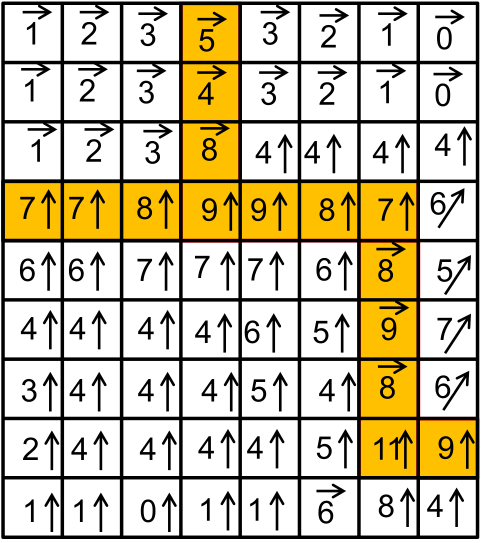
\includegraphics[width=.95\linewidth]{Picture/Canny}
\end{wrapfigure}
\textbf{Passo 3}: Costruiamo una prima approssimazione dei bordi, chiamiamo questa immagine $g_N(x,y)$ e inizializziamo tutti i suoi pixel a 0. Consideriamo i bordi come paralleli a 4 direzioni (verticali, orizzontali e le 2 diagonali), non ci interessa il verso ma solo la direzione. Dato il vettore gradiente del pixel $(x,y)$ in $f$ chiamiamo $d_k$ la direzione (tra le 4 definite prima) più prossima all'angolo del gradiente e $K = ||\nabla f_s||$ il modulo del gradiente. Se $K$ è minore di almeno uno fra i $||\nabla f_s||$
dei picel adiacenti a $(x,y)$ lungo la direzione $d_k$ allora $g(x,y) = 0$ altrimenti $g_N(x,y) = K$.

In questo modo individuiamo un solo punto per ogni bordo, man mano che il gradiente aumenta avvicinandosi al bordo stesso.

\textbf{Passo 4 hysteresis thresholding}: Consideriamo 2 soglie $T_H$ e $T_L$ in rapporto variabile (solitamente tra $2:1$ e  $3:1$) e costriuamo 2 imagini bordi forti $g_{NH}$ e  bordi deboli $g_{NL}$ utilizzando rispettivamente prima e seconda soglia.

In $g_{NH}$, avendo usato una soglia più alta, ci saranno meno pixel. Aggiorno $g_{NL}$ in modo che contenga solo i pixel che mancano a $g_{NH}$ in questo modo: $g_{NL}=g_{NL}-g_{NH}$. I Pixel in $g_{NH}$ vengono marcati tutti come validi, poi per riempire i buchi di questa maschera procedo come segue: 
\begin{enumerate}
	\item etichetto tutti i pixel di $g_{NH}$ come non visitati;
	\item per ogni pixel $(x,y)$ etichettato come non visitato:
	\begin{enumerate}
		\item etichetto come bordo valido tutti i pixel in $g_{NL}$ adiacenti a $(x,y)$;
		\item etichetto $(x,y)$ come visitato;
	\end{enumerate}
\end{enumerate}
Alla fine della procedura tutti i pixel etichettati come validi saranno considerati bordi.

\subsection{Line Detection}
